\documentclass[tikz]{standalone}
\usepackage{fontspec}
\renewcommand*{\familydefault}{\sfdefault}
\usepackage{standalone, amssymb}
\usetikzlibrary{arrows.meta, decorations.pathreplacing, shapes.geometric}
%\usetikzlibrary{positioning,fit,shapes.geometric,fadings,bayesnet}

\begin{document}

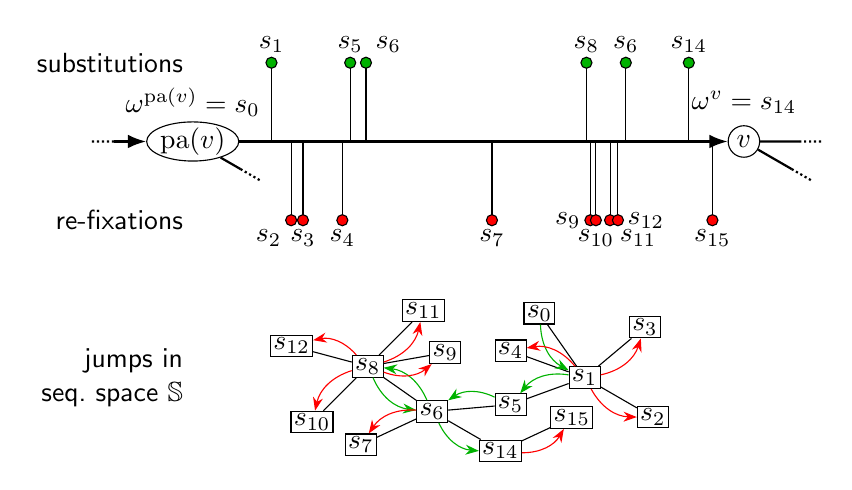
\begin{tikzpicture}[
%label position=0,
radius=2 pt,
treenode/.style={
ellipse,
draw,
minimum size=0.4 cm,
inner sep=0 pt,
}
]

% tree nodes
\node [treenode] at (0,0) (pa)
{\(\mathrm{pa}(v)\)};
\node [treenode] at (0:7 cm) (v)  {\(v\)};

\draw [thick, -Latex] (pa) -- (v);

% truncated edges
\draw[thick, solid]
(v) -- +(0:0.7 cm) coordinate(v1)
(v) -- +(-30:0.7 cm) coordinate(v2)
(pa) -- +(-30:0.7 cm) coordinate(w2)
;
\draw [thick, solid, -Latex] (180:1.0 cm) coordinate(pa2) -- (pa);
\draw[thick,densely dotted]
(v1) -- +(0:0.3 cm)
(v2) -- +(-30:0.3 cm)
(w2) -- +(-30:0.3 cm)
(pa2) -- ++(180:0.3 cm)
;

\path[align=right, anchor=east]
(pa) +(90:1) node {substitutions}
(pa) +(90:-1) node {re-fixations}
;

\path
% substitutions
(1,1) coordinate(t1)
(2,1) coordinate(t5)
(2.2,1) coordinate(t6)
(5,1) coordinate(t8)
(5.5,1) coordinate(t13)
(6.3,1) coordinate(t14)
% re-fixations
(1.25,-1) coordinate(t2)
(1.4,-1) coordinate(t3)
(1.9,-1) coordinate(t4)
(3.8,-1) coordinate(t7)
(5.05,-1) coordinate(t9)
(5.12,-1) coordinate(t10)
(5.3,-1) coordinate(t11)
(5.4,-1) coordinate(t12)
(6.6,-1) coordinate(t15)
;

% plot
\draw plot[ycomb, mark=*, mark options={draw=black, fill=green!70!black}] coordinates{
% substitutions
(t1) (t5) (t6) (t8) (t13) (t14)
};

% plot
\draw plot[ycomb, mark=*, mark options={draw=black, fill=red}] coordinates{
% re-fixations
(t2) (t3) (t4) (t7) (t9) (t10) (t11) (t12) (t15)
};

% labels for substitutions
\path[every node/.style={anchor=south}]
(t1) node {\(s_1\)}
(t5) node {\(s_5\)}
(t6) node[anchor=south west] {\(s_6\)}
(t8) node {\(s_8\)}
(t13) node {\(s_6\)}
(t14) node {\(s_{14}\)}
;

% labels for re-fixations
\path[every node/.style={anchor=north}]
(t2) node[anchor=north east] {\(s_2\)}
(t3) node {\(s_3\)}
(t4) node {\(s_4\)}
(t7) node {\(s_7\)}
(t9) node[anchor=east] {\(s_9\)}
(t10) node {\(s_{10}\)}
(t11) node[anchor=north west] {\(s_{11}\)}
(t12) node[anchor=west] {\(s_{12}\)}
(t15) node {\(s_{15}\)}
;

\path
(pa) +(90: 0.5 cm) node[anchor=center] {\(\omega^{\mathrm{pa}(v)}=s_0\)}
(v) +(90: 0.5 cm) node[anchor=center] {\(\omega^v=s_{14}\)}
;


% ``meanderings in sequence space''
\begin{scope}[xshift=0 cm, yshift=-3 cm]

\node[align=right, anchor=east] at (0,0) (S) {jumps in \\ seq.~space
\(\mathbb{S}\)};

\path[draw, every node/.style={draw, inner sep=1 pt}]
(S) ++(0:6 cm) node (s1) {\(s_1\)}
+(-30:1 cm) node (s2) {\(s_2\)}
+(40:1 cm) node (s3) {\(s_3\)}
+(160:1 cm) node (s4) {\(s_4\)}
++(-160:1 cm) node (s5) {\(s_5\)}
++(-175:1 cm) node (s6) {\(s_6\)}
+(-155:1 cm) node (s7) {\(s_7\)}
++(145:1 cm) node (s8) {\(s_8\)}
+(10:1 cm) node (s9) {\(s_9\)}
+(-135:1 cm) node (s10) {\(s_{10}\)}
+(45:1 cm) node (s11) {\(s_{11}\)}
+(165:1 cm) node (s12) {\(s_{12}\)}
(s6) % back mutation at t13
++(-30:1 cm) node (s14) {\(s_{14}\)}
+(25:1 cm) node (s15) {\(s_{15}\)}
(s1) +(125:1 cm) node (s0) {\(s_0\)}
;
\end{scope}

\draw
(s0) -- (s1)
(s1) -- (s2)
(s1) -- (s3)
(s1) -- (s4)
(s6) -- (s7)
(s8) -- (s9)
(s8) -- (s10)
(s8) -- (s11)
(s8) -- (s12)
(s14) -- (s15)
;

\draw
(s1) -- (s5)
(s5) -- (s6)
(s6) -- (s8)
(s6) -- (s14)
;

% jumps: substitutions
\draw[green!70!black, every edge/.style={draw, bend right, -Stealth}]
(s0) edge (s1)
(s1) edge (s5)
(s5) edge (s6)
(s6) edge (s8)
(s8) edge (s6)
(s6) edge (s14)
;

% jumps: re-fixations
\draw[red, every edge/.style={draw, bend right, -Stealth}]
(s1) edge (s2)
(s1) edge (s3)
(s1) edge (s4)
(s6) edge (s7)
(s8) edge (s9)
(s8) edge (s10)
(s8) edge (s11)
(s8) edge (s12)
(s14) edge (s15)
;

\end{tikzpicture}
\end{document}

